\documentclass[t,12pt]{beamer}

\usepackage{fontspec}

\usepackage{xunicode}
\usepackage{xltxtra}

\usepackage{polyglossia}

\setmainfont{Liberation Serif}
\newfontfamily\devanagarifont{Lohit Nepali}

\setmainlanguage{english}
\setotherlanguages{sanskrit}


\usepackage{graphicx}
\usepackage{color}
\usepackage{url}
\usepackage{textpos}
\usepackage{xspace}
\usepackage{array}
\usepackage[normalem]{ulem}

\newcommand\misspelt{\bgroup\markoverwith
{\textcolor{red}{\lower3.5pt\hbox{\sixly \char58}}}\ULon}
\DeclareRobustCommand{\fuuuuu}[1]{\texorpdfstring{\misspelt{#1}}{#1}}


\graphicspath{{./fig/}}

% theme options: hy/ml/hum, rovio/sinetti, hiit
% default: hy,rovio

%\usetheme[hy]{HY}
%\usetheme[hy,sinetti]{HY}
\usetheme[hum,rovio]{HY}
%\usetheme[ml,rovio]{HY}
%\usetheme[ml,rovio,hiit]{HY}


\title{State-of-the-art in Weighted Finite-State Spell-Checking\\
\scriptsize{CICLING 2014, \devanagarifont{काठमाडौं}}}

\author{\fuuuuu{Tommi A Pirinen} \and Krister Lindén
\scriptsize \guilsinglleft{}firstname.lastname@helsinki.fi\guilsinglright{}} 
\institute{University of Helsinki\\Department of Modern Languages}
\date{\today}

\begin{document}

\selectlanguage{english}

\HyTitle
%\maketitle


\section{Introduction}

       
\begin{frame}
    \frametitle{Spell-Checking}
    \begin{itemize}
        \item Spell-Checking is everywhere: browsers, office software, mobile
            phones, \ldots
        \item Three tasks: for each word \begin{enumerate}
                \item detect if word is correctly written / how likely the
                    written word is what was meant (language modelling
                    for error detection)
                \item if not, what modifications can be made to find more
                    likely correct word (error modelling)
                \item rank corrections in order of likelihood
                    (language modelling for error correction)
            \end{enumerate}
        \item Example: 1) cta 2) swap adjacent letters 3) Did you mean: cat?
    \end{itemize}
\end{frame}

\begin{frame}
    \frametitle{Spell-Checking and State-of-the-Art}
    \begin{itemize}
        \item State of the art as we know it: \begin{itemize}
                \item non-commercial use: hunspell (limited edit distance, no statistics)
                     correct, bayspell, etc. (statistics, linguistic analysis)
                \item commercial products (frequency word-form lists?);
                \item grammar checkers: LanguageTool, ... (context-based \(n\) gram
            models, programmatic rules)
    \end{itemize}
        \item Three tests to measure and motivate this: \begin{enumerate}
                \item coverage of the dictionary
                \item accuracy of corrections
                \item speed of spelling and correcting
            \end{enumerate}
    \end{itemize}
\end{frame}

\begin{frame}
    \frametitle{Test Data and Methods}
    \begin{itemize}
        \item All tests were tested on Wikipedia data, it is the only free
            open source corpus source for many languages
        \item The language models / dictionaries are from internet free open
            source repository in \url{http://giellatekno.uit.no} except English
            which is from P. Norvig
        \item The size and quality of Wikipedias varies: English data is
            huge, Finnish is large-ish and North Saami tiny and low-quality
            (written by non-native students) and Greenlandic even more so

        \item We scraped some spelling errors with corrections from
            Wikipedia change logs
    \end{itemize}
\end{frame}

\begin{frame}[label=links]
    \frametitle{Reproducible and usable spell-checking}
    \begin{itemize}
        \item Get it for LibreOffice (Mac OS X and Windows):
            \url{http://divvun.no/libreofficeoxt.html}
        \item Compile it for LibreOffice, enchant (works on nearly all
            reasonable Linux software):
            \url{https://sourceforge.net/projects/hfst/files/spell-transducers/}
        \item Reproduce experiments, try it out for your language, \ldots:
            \url{https://github.com/flammie/purplemonkeydishwasher/tree/master/2014-cicling}
    \end{itemize}
\end{frame}

\section{Tests for the State-of-the-Art}

\begin{frame}
    \frametitle{Coverage}
    \begin{itemize}
        \item Finite-state methods are well established in morphological
            dictionary writing / language modelling (cf. \emph{Two-level
            morphology} Koskenniemi (1983); \emph{Finite-State Morphology}
            Karttunen and Beesley (2003), \ldots)
        \item Naive coverage tests presented in the paper shows greatly
            larger coverage for Finnish
        \item Greenlandic has not been shown with non-finite state methods
            beyond some 25 \% coverage (from newspaper text,
            according to my colleagues at
            \url{oqaaserpassualeriffik.org})
    \end{itemize}
\end{frame}

\begin{frame}
    \frametitle{Coverage Results}
    Naive coverage = proportion of tokens with > 0 analyses\\
    \begin{tabular}{l|r}
        Language Model & Coverage \\
        English aspell & 22.7 \\
        English WFSA & 80.1 \\
        Finnish WFSA & 64.8 \\
        North Saami Hunspell & 34.4 \\
        North Saami WFSA & 48.5 \\
        Greenlandic WFSA & 25.3 \\
    \end{tabular}\\
    The naive coverage figures give some idea of the starting point for
    spelling checker and the corpus data quality. Note that Wikipedia tokens
    has a lot of rubbish for spelling correction.
\end{frame}

\begin{frame}
    \frametitle{Accuracy}
    \begin{itemize}
        \item Tested on the wikipedia's errors as logged by real users with
            some conventional comment
        \item Only solvable errors (target word-form in dictionary)
        \item Improvement in 1st guess correct and cumulative corrections
            for all langauges
        \item Likely because of addition of word form frequency statistics
    \end{itemize}
\end{frame}

\begin{frame}
    \frametitle{Accuracy Results}
    Quality = Proportion of correct suggestions at given position\\
    \begin{tabular}{l|rr}
        Language Model & $1^{st}$ & $2^{nd}$ \\
        English aspell &55.7 & 5.7 \\
        English Hunspell &59.3 & 5.8 \\
        English WFSA &66.7 & 7.0 \\
 \hline 
 Finnish aspell & 21.1 & 5.8 \\ 
 Finnish WFSA  & 54.8 & 19.0 \\
\end{tabular}\\
Less resourced languages' scarce error data is further discussed in the paper
\end{frame}

\begin{frame}
    \frametitle{Speed}
    \begin{itemize}
        \item Easy measure, fed wikipedia data to command line spell-checkers
            and measured throughput
        \item Two test sets: all data (real world speed) and only known
            misspellings (correction speed)
        \item Beats Hunspell on all measures, aspell is still fastest though
    \end{itemize}
\end{frame}

\begin{frame}
    \frametitle{Speed Results}
    Speed = tokens processed per second (raw data), Memory = peak resident stack
    size\\
    \begin{tabular}{l|rr}
        Language Model & WPS & Memory in MB\\
        \hline
       English Hunspell & 74 & 7.5 \\
       English aspell & 20,000 & 1.3 \\
       English WFSA & 5,721 & 7.0 \\
        \hline
        North Saami Hunspell & 3 & 151.0 \\
       North Saami WFSA & 5,025 & 31.4 \\
        \hline
        Greenlandic WFSA & 85 & 300.7 \\
    \end{tabular}\\
\end{frame}

\begin{frame}
    \frametitle{Conclusion}
    \begin{itemize}
        \item Our WFST spell-checking beats de facto standard open source
            systems on speed, accuracy and coverage
        \item It is a speed to quality trade-off, this experiment shows we can
            tune the parameters to optimise all aspects
        \item We have available usable spell-checkers for numerous languages
        (
        \iffalse
        \hyperlink{links}{\beamergotobutton{Links}}
        \fi
        \iftrue
        cf. links slide
        \fi)
            and can generate more given a corpus or dictionary data in some
            palatable format (e.g. Beesley Karttunen FSM, freq. lists,
            hunspell, apertium monodix...)
    \end{itemize}
\end{frame}

\section{The last slide section}

\begin{frame}
    \frametitle{Thanks kiitos \devanagarifont{ धेरै धेरै धन्यबाद}}
    Questions?
    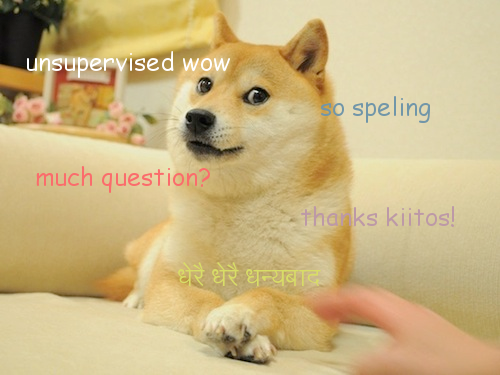
\includegraphics[width=\textwidth]{questions-doge}
\end{frame}

\begin{frame}
    \frametitle{Reproducible and usable spell-checking}
    \begin{itemize}
        \item Get it for LibreOffice (Mac OS X and Windows):
            \url{http://divvun.no/libreofficeoxt.html}
        \item Compile it for LibreOffice, enchant (works on nearly all
            reasonable Linux software):
            \url{https://sourceforge.net/projects/hfst/files/spell-transducers/}
        \item Reproduce experiments, try it out for your language, \ldots:
            \url{https://github.com/flammie/purplemonkeydishwasher/tree/master/2014-cicling}
    \end{itemize}
\end{frame}

\end{document}
% vim: set spell:
